% Auto-generated by the analysis pipeline — do not edit
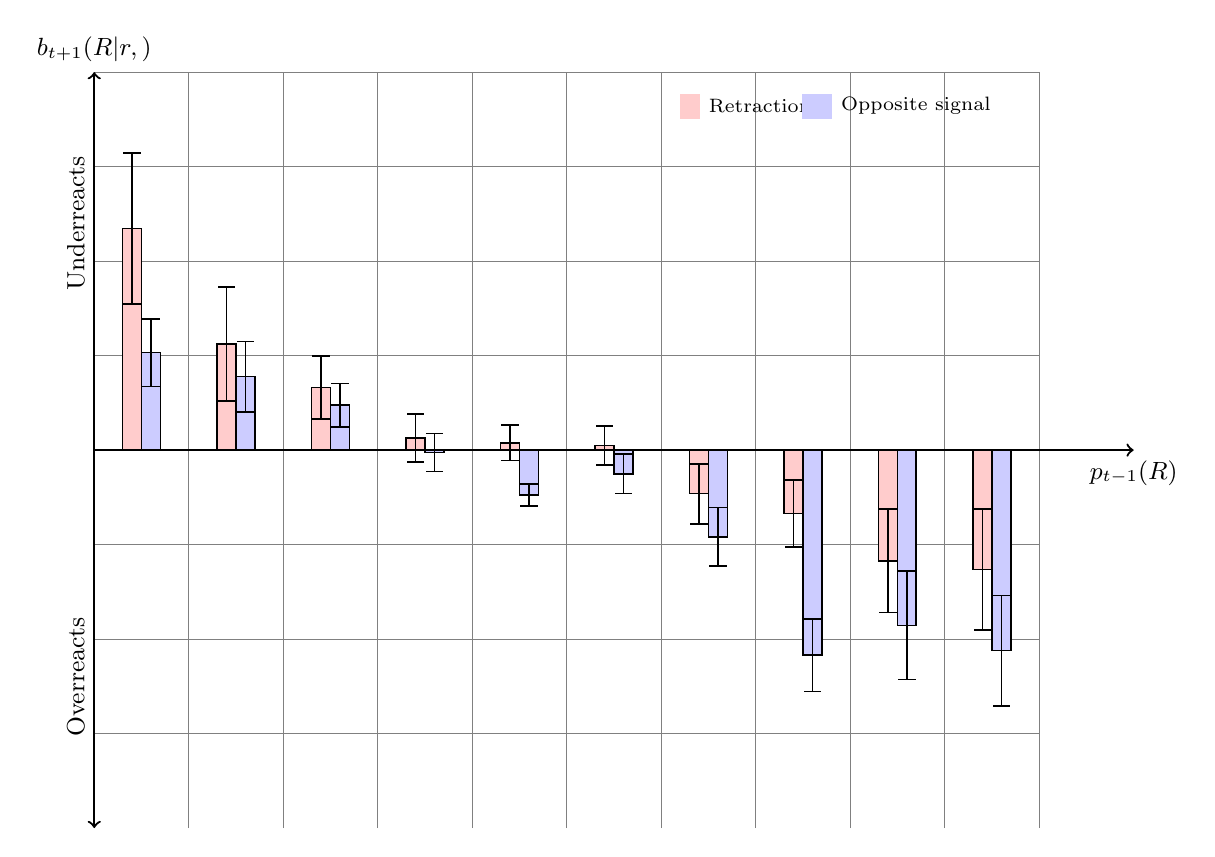
\begin{tikzpicture}[scale=12]
\draw[help lines,step=0.1] (0,-0.4) grid (1,0.4);
\filldraw[opaque,white!80!red] (0.0300,0) rectangle (0.0500,0.2345);
\draw[line width=0.6] (0.0300,0) rectangle (0.0500,0.2345);
\draw[line width=0.6,|-|] (0.0400,0.1537) -- (0.0400,0.3152);
\filldraw[opaque,white!80!blue] (0.0500,0) rectangle (0.0700,0.1031);
\draw[line width=0.6] (0.0500,0) rectangle (0.0700,0.1031);
\draw[line width=0.6,|-|] (0.0600,0.0665) -- (0.0600,0.1397);
\filldraw[opaque,white!80!red] (0.1300,0) rectangle (0.1500,0.1122);
\draw[line width=0.6] (0.1300,0) rectangle (0.1500,0.1122);
\draw[line width=0.6,|-|] (0.1400,0.0511) -- (0.1400,0.1732);
\filldraw[opaque,white!80!blue] (0.1500,0) rectangle (0.1700,0.0777);
\draw[line width=0.6] (0.1500,0) rectangle (0.1700,0.0777);
\draw[line width=0.6,|-|] (0.1600,0.0395) -- (0.1600,0.1158);
\filldraw[opaque,white!80!red] (0.2300,0) rectangle (0.2500,0.0661);
\draw[line width=0.6] (0.2300,0) rectangle (0.2500,0.0661);
\draw[line width=0.6,|-|] (0.2400,0.0320) -- (0.2400,0.1001);
\filldraw[opaque,white!80!blue] (0.2500,0) rectangle (0.2700,0.0475);
\draw[line width=0.6] (0.2500,0) rectangle (0.2700,0.0475);
\draw[line width=0.6,|-|] (0.2600,0.0237) -- (0.2600,0.0712);
\filldraw[opaque,white!80!red] (0.3300,0) rectangle (0.3500,0.0126);
\draw[line width=0.6] (0.3300,0) rectangle (0.3500,0.0126);
\draw[line width=0.6,|-|] (0.3400,-0.0136) -- (0.3400,0.0388);
\filldraw[opaque,white!80!blue] (0.3500,0) rectangle (0.3700,-0.0025);
\draw[line width=0.6] (0.3500,0) rectangle (0.3700,-0.0025);
\draw[line width=0.6,|-|] (0.3600,-0.0236) -- (0.3600,0.0186);
\filldraw[opaque,white!80!red] (0.4300,0) rectangle (0.4500,0.0077);
\draw[line width=0.6] (0.4300,0) rectangle (0.4500,0.0077);
\draw[line width=0.6,|-|] (0.4400,-0.0120) -- (0.4400,0.0274);
\filldraw[opaque,white!80!blue] (0.4500,0) rectangle (0.4700,-0.0478);
\draw[line width=0.6] (0.4500,0) rectangle (0.4700,-0.0478);
\draw[line width=0.6,|-|] (0.4600,-0.0604) -- (0.4600,-0.0352);
\filldraw[opaque,white!80!red] (0.5300,0) rectangle (0.5500,0.0048);
\draw[line width=0.6] (0.5300,0) rectangle (0.5500,0.0048);
\draw[line width=0.6,|-|] (0.5400,-0.0166) -- (0.5400,0.0261);
\filldraw[opaque,white!80!blue] (0.5500,0) rectangle (0.5700,-0.0252);
\draw[line width=0.6] (0.5500,0) rectangle (0.5700,-0.0252);
\draw[line width=0.6,|-|] (0.5600,-0.0469) -- (0.5600,-0.0035);
\filldraw[opaque,white!80!red] (0.6300,0) rectangle (0.6500,-0.0461);
\draw[line width=0.6] (0.6300,0) rectangle (0.6500,-0.0461);
\draw[line width=0.6,|-|] (0.6400,-0.0788) -- (0.6400,-0.0135);
\filldraw[opaque,white!80!blue] (0.6500,0) rectangle (0.6700,-0.0917);
\draw[line width=0.6] (0.6500,0) rectangle (0.6700,-0.0917);
\draw[line width=0.6,|-|] (0.6600,-0.1235) -- (0.6600,-0.0598);
\filldraw[opaque,white!80!red] (0.7300,0) rectangle (0.7500,-0.0672);
\draw[line width=0.6] (0.7300,0) rectangle (0.7500,-0.0672);
\draw[line width=0.6,|-|] (0.7400,-0.1035) -- (0.7400,-0.0310);
\filldraw[opaque,white!80!blue] (0.7500,0) rectangle (0.7700,-0.2170);
\draw[line width=0.6] (0.7500,0) rectangle (0.7700,-0.2170);
\draw[line width=0.6,|-|] (0.7600,-0.2564) -- (0.7600,-0.1776);
\filldraw[opaque,white!80!red] (0.8300,0) rectangle (0.8500,-0.1171);
\draw[line width=0.6] (0.8300,0) rectangle (0.8500,-0.1171);
\draw[line width=0.6,|-|] (0.8400,-0.1726) -- (0.8400,-0.0616);
\filldraw[opaque,white!80!blue] (0.8500,0) rectangle (0.8700,-0.1855);
\draw[line width=0.6] (0.8500,0) rectangle (0.8700,-0.1855);
\draw[line width=0.6,|-|] (0.8600,-0.2438) -- (0.8600,-0.1273);
\filldraw[opaque,white!80!red] (0.9300,0) rectangle (0.9500,-0.1265);
\draw[line width=0.6] (0.9300,0) rectangle (0.9500,-0.1265);
\draw[line width=0.6,|-|] (0.9400,-0.1913) -- (0.9400,-0.0617);
\filldraw[opaque,white!80!blue] (0.9500,0) rectangle (0.9700,-0.2121);
\draw[line width=0.6] (0.9500,0) rectangle (0.9700,-0.2121);
\draw[line width=0.6,|-|] (0.9600,-0.2714) -- (0.9600,-0.1529);
\draw[line width=0.8,->]  (0,0) -- (1.1,0) node[below] {\small{$p_{t-1}(R)$}};
\draw[line width=0.8,<->] (0,-0.4) -- (0,0.4) node[above] {\small{$b_{t+1}(R|r,\xmark)$}};
\draw (0,0.24) node[above,rotate=90] {\small{Underreacts}};
\draw (0,-0.24) node[above,rotate=90] {\small{Overreacts}};
\filldraw[white!80!red] (0.62,0.3510) rectangle (0.64,0.3760);
\node[right] at (0.64,0.3640) {\scriptsize{Retraction}};
\filldraw[white!80!blue] (0.75,0.3510) rectangle (0.78,0.3760);
\node[right] at (0.78,0.3640) {\scriptsize{Opposite signal}};
\end{tikzpicture}
